Zur Messung der Dispersion wird folgender Versuchsaufbau verwendet:
\begin{figure}[h!]
  \centering
  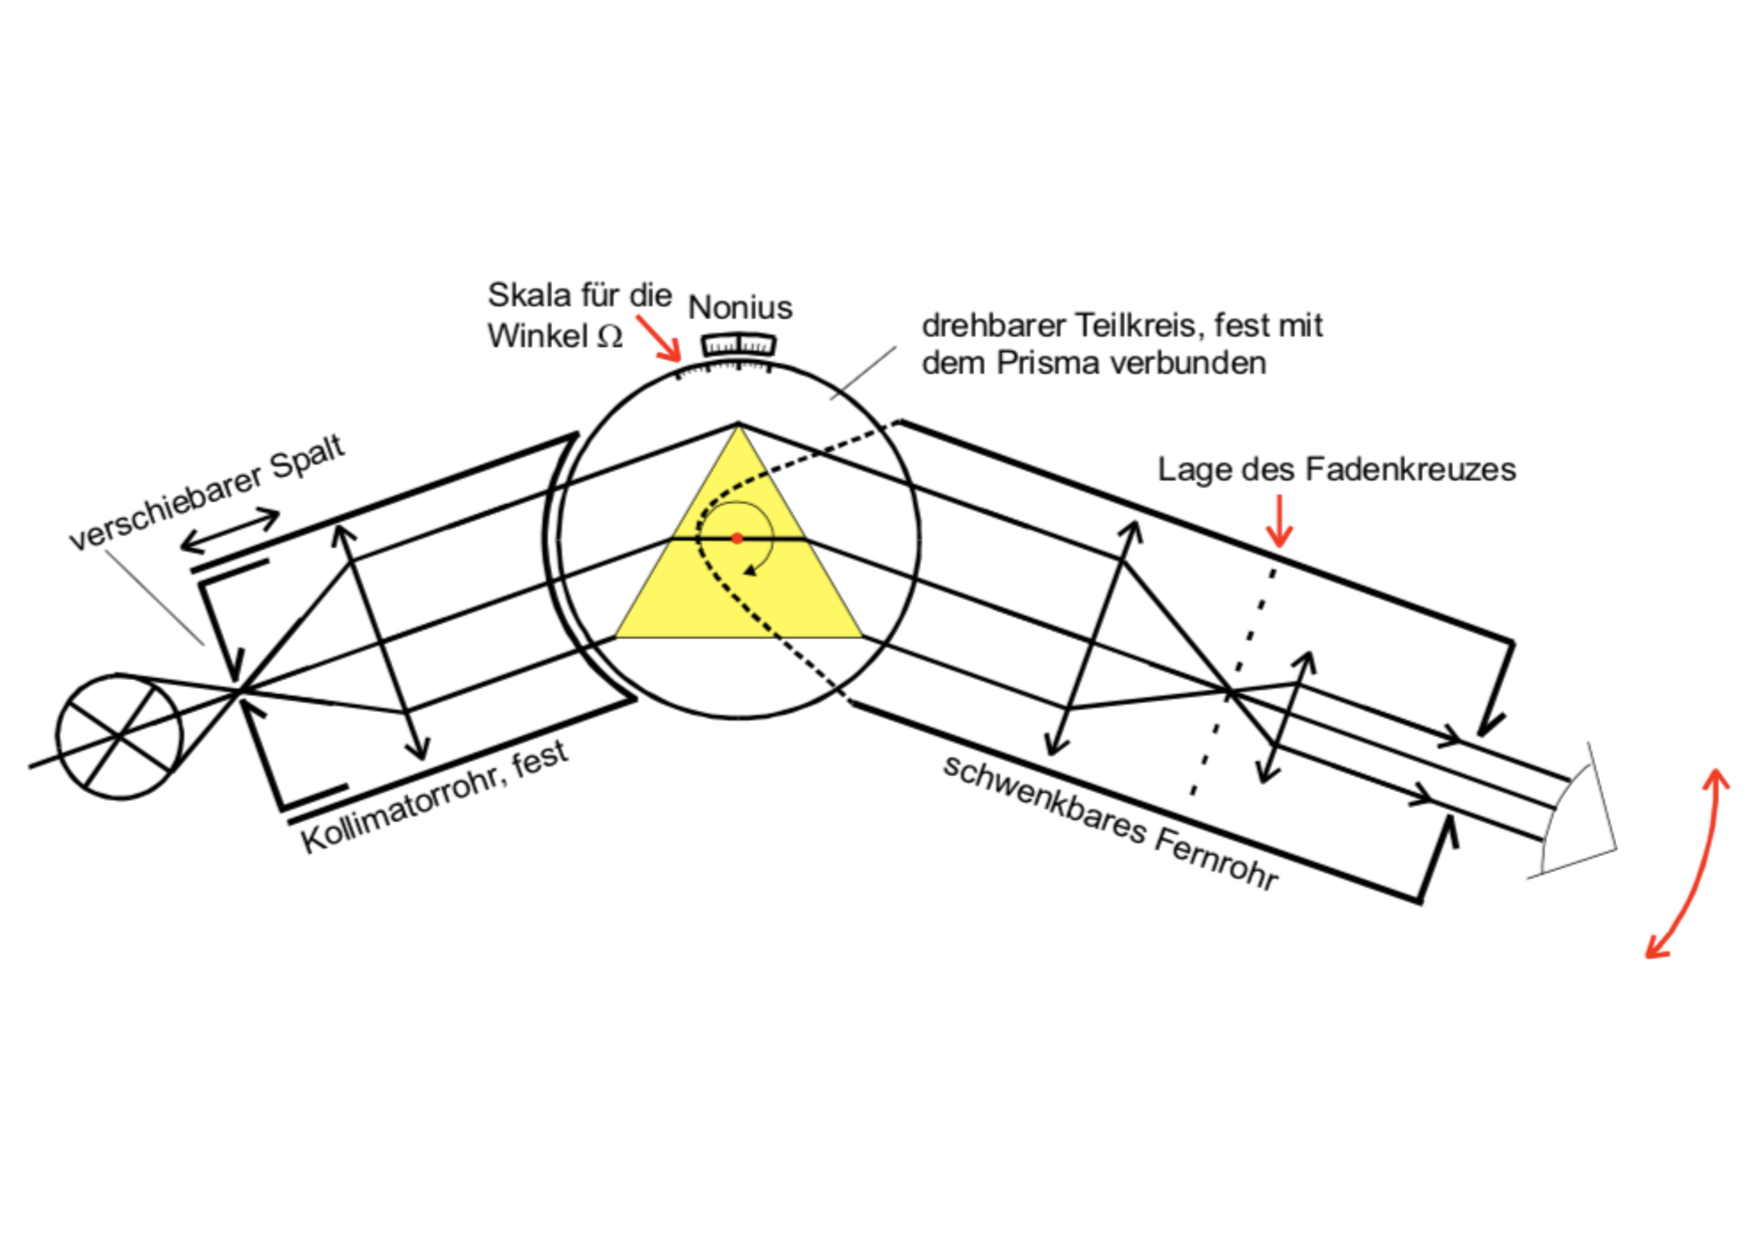
\includegraphics[width=\textwidth]{aufbau.pdf}
  \caption{Versuchsaufbau \cite{1}}
  \label{fig:aufbau}
\end{figure}
Eine Hg-Cd-Spektrallampe wirft ihr Licht durch einen Spalt in ein Kollimatorrohr.
Das Kollimatorrohr macht aus den Lichtstrahlen parallele Strahlen.
Die Strahlen treffen dann auf das Glasprisma auf einer drehbaren Scheibe (Goniometerscheibe) mit einer Skala zum Ablesen des Winkels.
Daraufhin treffen die Strahlen auf ein Fernglas mit Fadenkreuz, welches schwenkbar an der Aufhängung des Prismas montiert ist.
So kann jeder Winkel um das Prisma auf Lichtstrahlen untersucht werden.
%phi messung
\\Zur Messung des Winkels $\varphi$ wird das Prisma mit der markierten Ecke in Richtung der Lichtquelle gestellt.
Die Null-Markierung der Winkelskala wird in einem $\SI{45}{°}$-Winkel links zum Kollimatorrohr gelegt (Abb. \ref{fig:phimessung}).
\begin{figure}[h!]
  \centering
  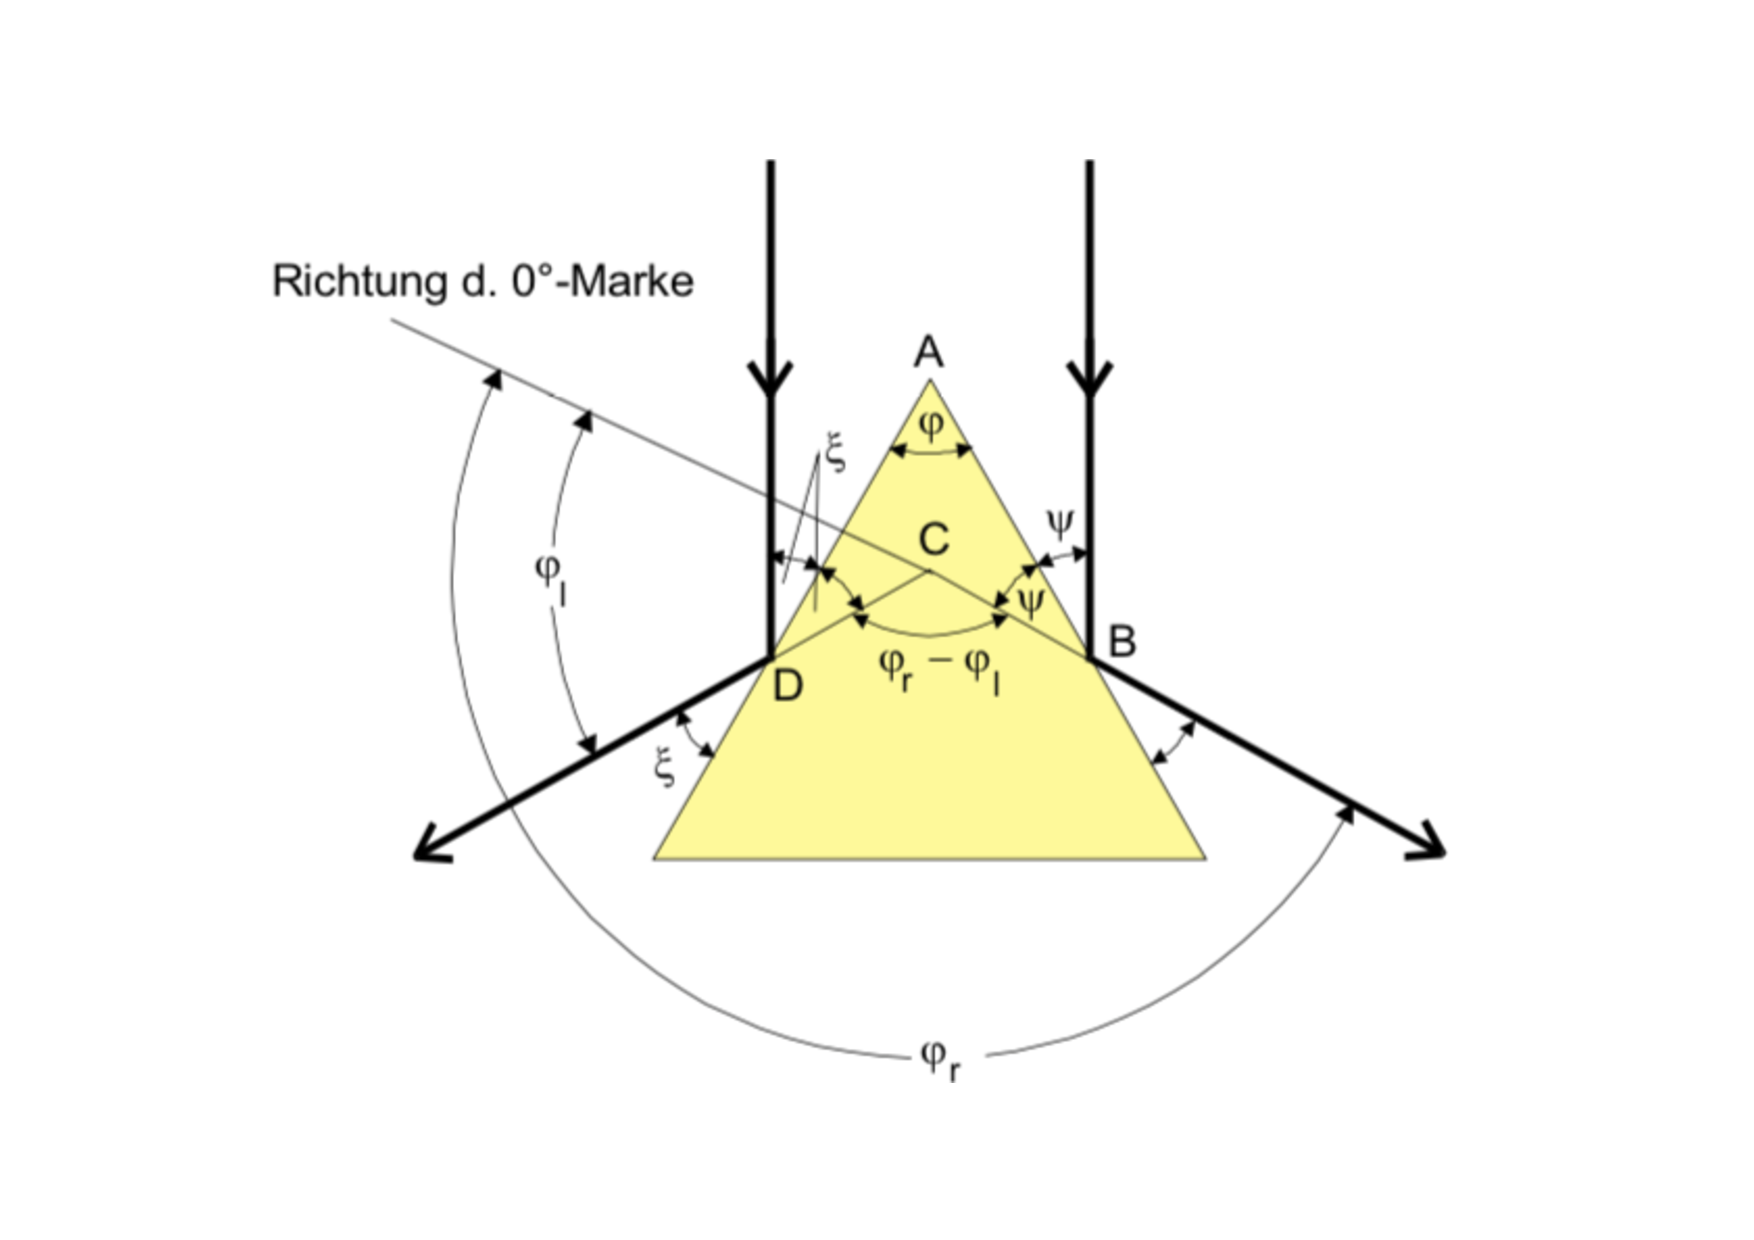
\includegraphics[width=0.8\textwidth]{phimessung.pdf}
  \caption{Strahlengang zur $\varphi$-Messung \cite{1}}
  \label{fig:phimessung}
\end{figure}
Der Strahl wird auf beiden Seiten des Prismas reflektiert.
Da die Strahlen parallel sind, ergibt sich folgende Gleichung für $\varphi$:
\begin{align}
  \varphi= \frac{1}{2} (\varphi_{\text{r}} - \varphi_{\text{l}}).
\end{align}
Die beiden Winkel $\varphi_{\text{l}}$ und $\varphi_{\text{r}}$ werden gemessen.
%eta Messung
\\Der $\eta$-Messung liegt folgende Abbildung (Abb. \ref{fig:etamessung1}) zugrunde:
\begin{figure}[h!]
  \centering
  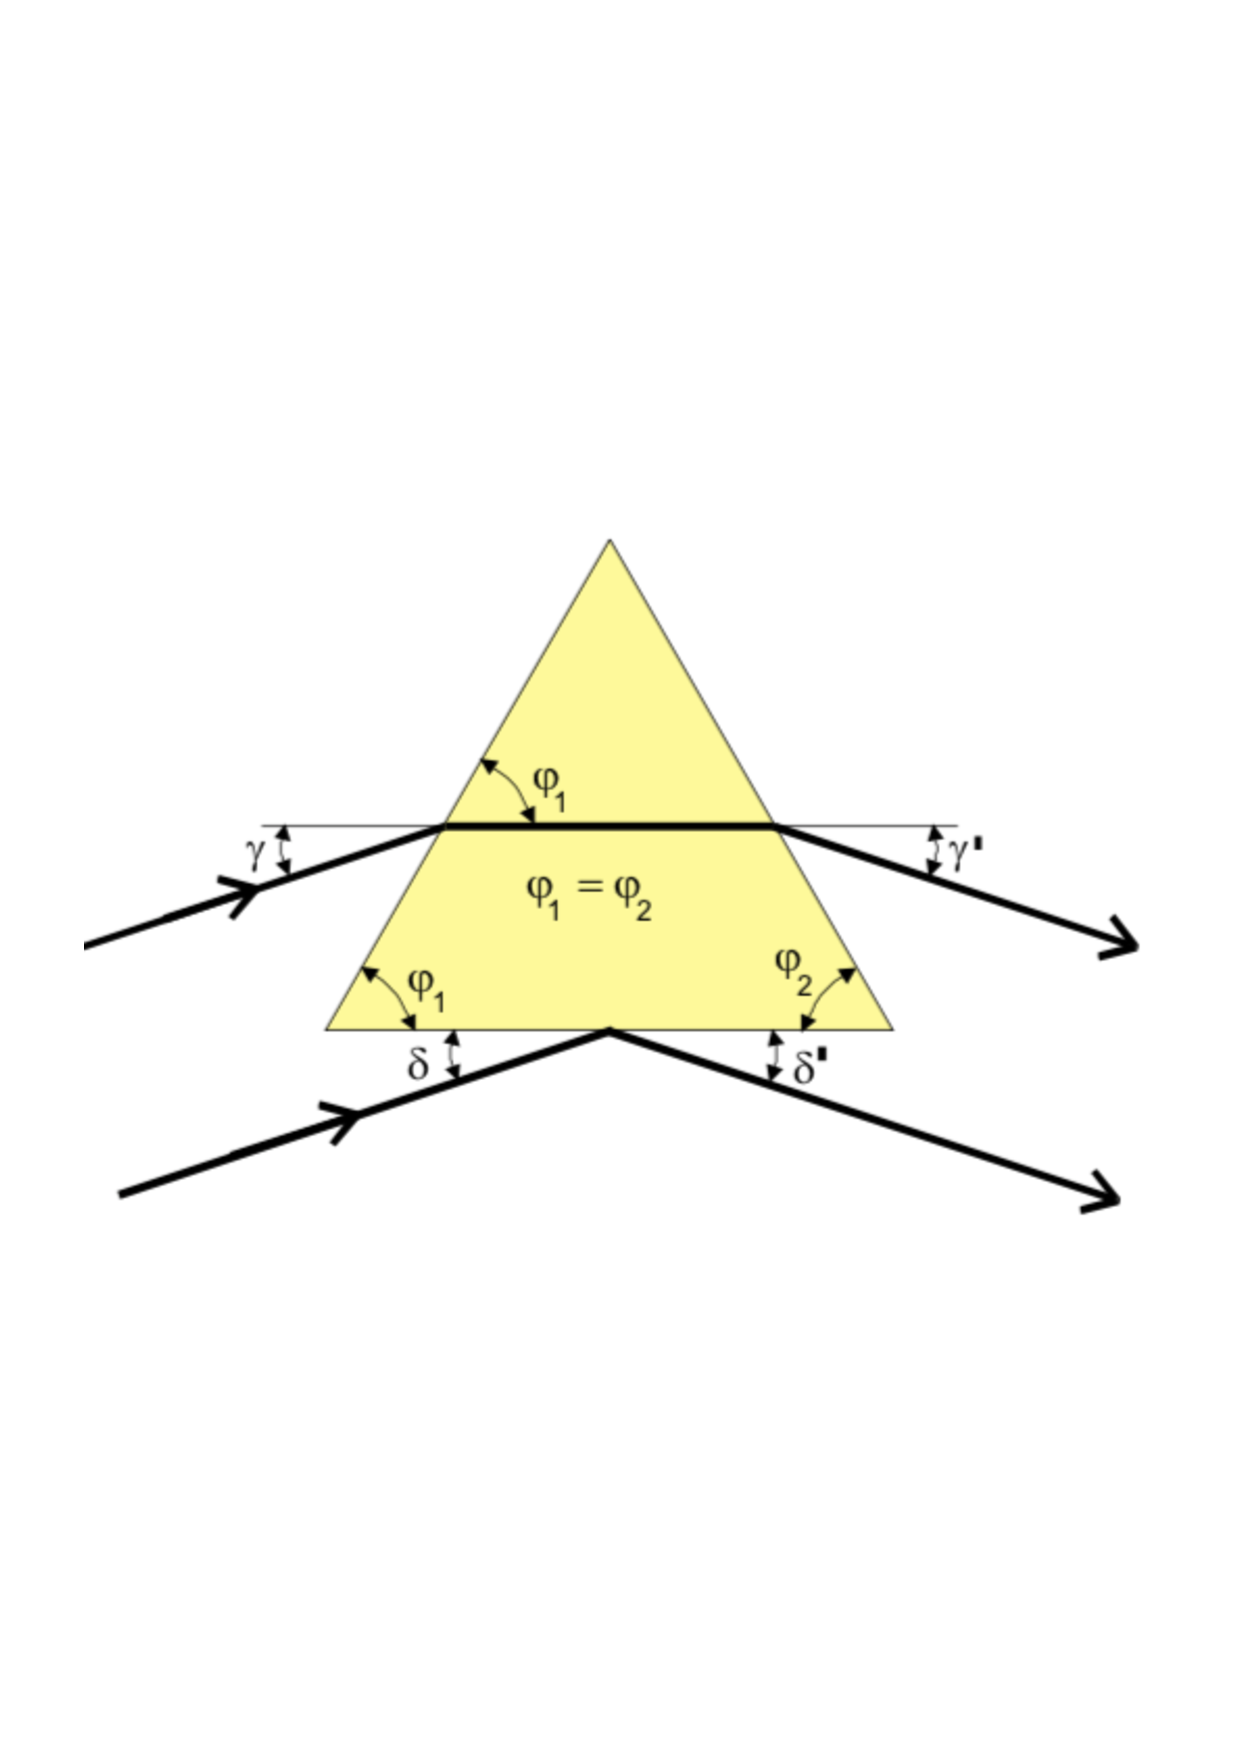
\includegraphics[width=0.8\textwidth]{etamessung1.pdf}
  \caption{Strahlengang zur $\eta$-Messung \cite{1}}
  \label{fig:etamessung1}
\end{figure}
Der Lichtstrahl wird einerseits reflektiert (unterer Strahl), andererseits gebrochen (oberer Strahl).
Wenn der Strahlengang symmetrisch ist, sind auch die ausfallenden Strahlen parallel.
Der symmetrische Strahlengang ergibt sich, wenn die reflektierten und die gebrochenen Strahlenanteile aufeinanderfallen.
Dazu wird die Goniometerscheibe beim Betrachten des Spektrums gedreht, bis sich die reflektierte, weiße Linie mit den jeweiligen Linien des Spektrums überlagert.
Die Messung wird für beide Seiten des Prismas durchgeführt:
\begin{figure}[h!]
  \centering
  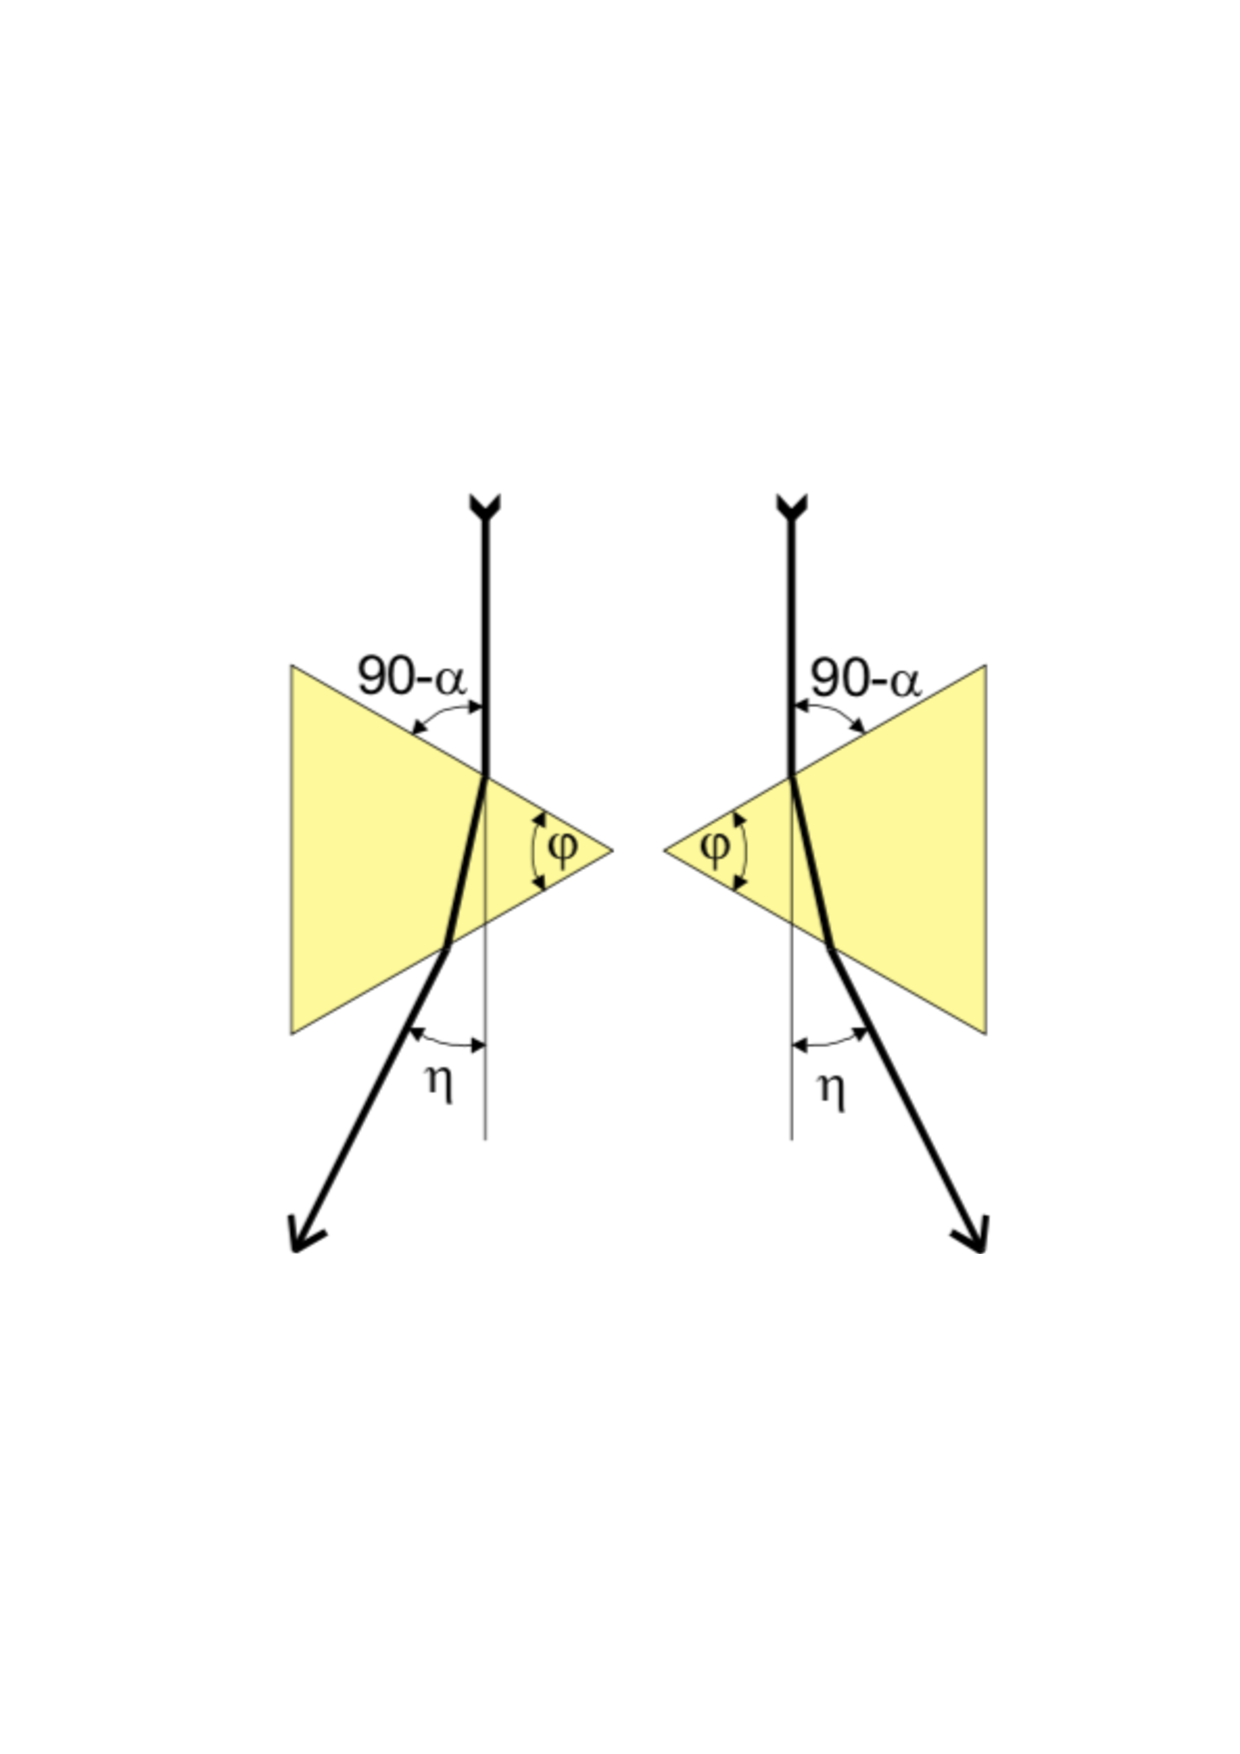
\includegraphics[width=0.8\textwidth]{etamessung2.pdf}
  \caption{Symmetrischer Strahlengang der $\eta$-Messung \cite{1}}
  \label{fig:etamessung2}
\end{figure}
Aus den Winkelbeziehungen der Abbildungen \ref{fig:etamessung1} und \ref{fig:etamessung2} folgt die Gleichung für den Winkel $\eta$:
\begin{align}
  \eta= 180 - (\Omega_{\text{r}} - \Omega_{\text{l}}).
\end{align}
Die gemessenen Winkel sind in Abbildung \ref{fig:etamessung3} zu sehen:
\begin{figure}[h!]
  \centering
  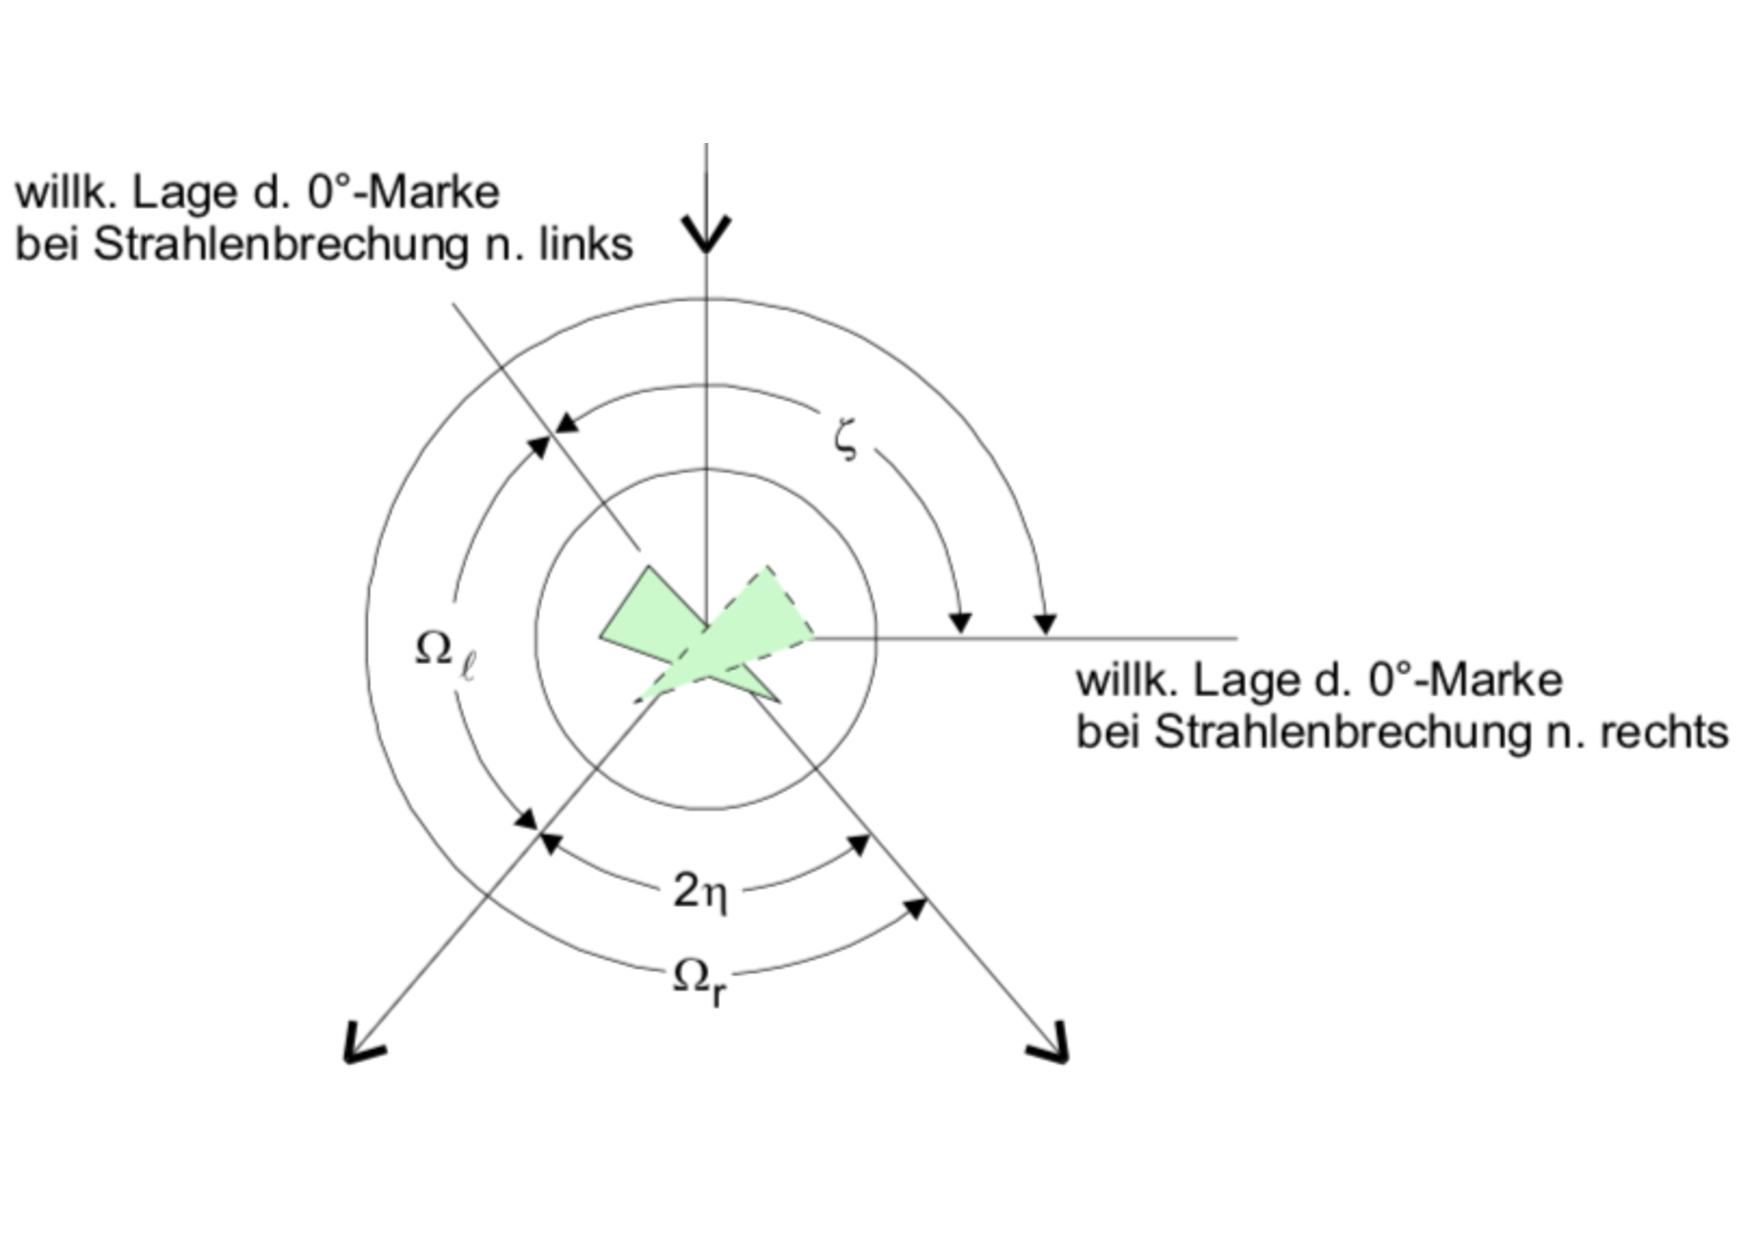
\includegraphics[width=\textwidth]{etamessung3.pdf}
  \caption{Gemessene Winkel der $\eta$-Messung \cite{1}}
  \label{fig:etamessung3}
\end{figure}
Dazu wird das Prisma zunächst mit der markierten Ecke in einen $\SI{135}{°}$-Winkel rechts zur Lichtquelle gedreht, so dass das Licht zuerst durch die rückwärtige Seite des Prismas fällt.
Dann wird der Winkel $\Omega_{\text{r}}$ abgelesen für die jeweiligen Spektrallinien.
Anschließend wird die Goniometerscheibe gedreht, bis das Prisma in einem Winkel von ca. $\SI{135}{°}$ links zur Lichtquelle steht.
Es wird der Winkel $\Omega_{\text{l}}$ für alle Spektrallinien gemessen.
\FloatBarrier
